In order to complete this guide you will need the following equipment.

\begin{enumerate}
\item Laptop with the following: 
\begin{enumerate}
\item The \gls{sdr} Drivers. These are usually available from the manufacturers website.
\item The Arduino IDE\footnote{https://www.arduino.cc/en/Main/Software}.
\item The RadioHead-Extras library should be installed and made available to the Arduino IDE. The library is in the \verb|src| folder of this repo.
\item gnuradio\footnote{https://www.gnuradio.org}.
\item A clone of this repo and performed recursively\footnote{git clone --recursive https://github.com/geekskick/wex-guide}.
\end{enumerate}
\item An SDR with an appropriate antenna for looking at the 430-440MHz frequency range. Its up to you which you use, there are loads available for a reasonable price\footnote{https://www.rtl-sdr.com}.
\item Two Adafruit Feathers with an RFM69 packet radio module attached\footnote{https://learn.adafruit.com/adafruit-feather-m0-radio-with-rfm69-packet-radio/overview} as shown in \cref{adafruit}. These should ideally have antennas attached as described in the Adafruit documentation\footnote{https://learn.adafruit.com/adafruit-feather-m0-radio-with-rfm69-packet-radio/antenna-options}. 

\centrefigurestart
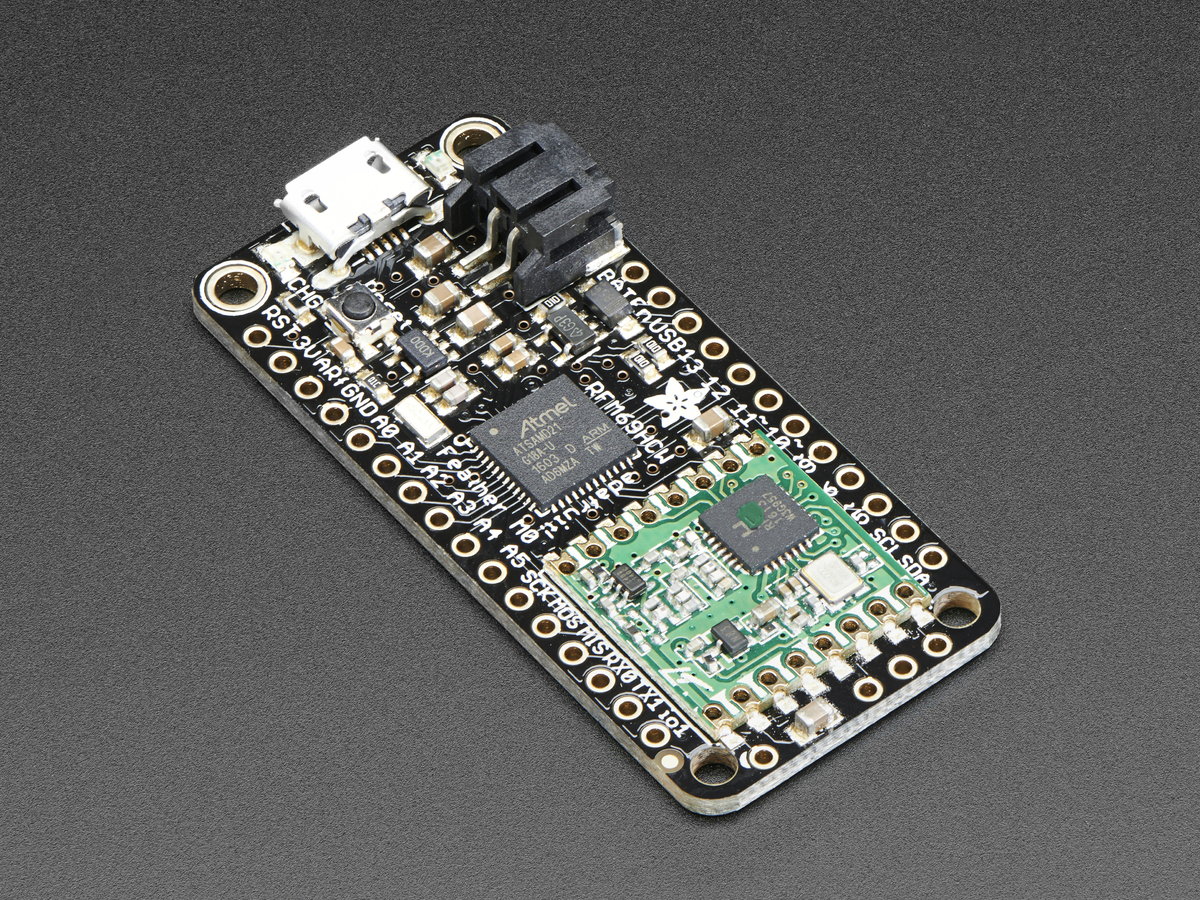
\includegraphics[width=\imgwidth]{feather.jpg}
\caption{An Adafruit Feather M0 with RFM69 Packet Radio}
\label{adafruit}
\centrefigureend

\end{enumerate}